\documentclass[11 pt]{article}
\usepackage{amsmath, amssymb, color, xcolor}
\usepackage{graphicx}
\usepackage{fullpage}
\usepackage[hidelinks]{hyperref}
\usepackage{tikz}
\usetikzlibrary{arrows.meta, shapes}
\usepackage{caption, subcaption}
\usepackage{natbib} % gives us \citet: Author (year) and \citep: (Author; year)
\usepackage{authblk}
\newcommand{\plr}[1]{{\color{blue}\it #1}}
\newcommand{\jss}[1]{{\color{olive}\it #1}}
% \newcommand{\ddt}{\frac{d}{dt}}
\newcommand{\ddt}{\dot}
\newcommand{\ro}{{ro}}
\newcommand{\nro}{{\bar{r}o}}
\newcommand{\rno}{{r\bar{o}}}
\newcommand{\nrno}{{\bar{r}\bar{o}}}
\newcommand{\reachable}{\mathcal{R}}
\newcommand{\unobservable}{\bar{\mathcal{O}}}
\newcommand{\R}{\mathbb{R}}
\newcommand{\E}{\mathbb{E}}
\renewcommand{\P}{\mathbb{P}}

\DeclareMathOperator{\spn}{span}

\newtheorem{theorem}{Theorem}
\newtheorem{lemma}{Lemma}
\newtheorem{definition}{Definition}
\newtheorem{example}{Example}

\begin{document}

\paragraph{To do, soon:}

\begin{enumerate}
    \item Add biology to introduction. (keep an eye out for concrete numbers we can use!)

    \item Do some order-of-magnitude calculation to figure out how fast systems should drift.

    \item Write out simple examples in biological words.

    \item Rephrase hybrid inviability example in biological terms.  Discuss F1's (or heterozygotes) versus F2's.

    \item Clarify our assumptions around $x(0)$. 

    \item Note we don't include $D$ for simplicity but don't.

    \item Figure out how to specify $P$ for Kalman decomposition.

    \item Prove or find citation for uniqueness of minimal system up to basis change.

    \item Work examples (minimal; not minimal; with/without B,C fixed) of Kalman decomposition and description of moving along the walk.

    \item Write down and decide between options for parameterizing the random walk on the neutral manifold:
        use Kalman decomposition, and parameterize Brownian motion so that it has constant speed;
        OR consider Josh's parameteriziation like this;
        OR just say we do Brownian motion on the manifold (more or less implicit characterization).

    \item Consider options for fitness function: Euclidean? Sign of eigenvalues?  Time domain or frequency?
        First try on simple concrete examples.

    \item Describe model leading to constraints on regulation so we have a stationary distribution.
        Ask questions of stationary distribution: robustness, connectivity, xxx?

    \item Write something in discussion about nonlinear systems.  Do an example if there is a feasible one.

\end{enumerate}

% Outline:
% 
% - What the problems are:
% 
%     * evolution of perfectly fit populations
% 
% - Motivations: Can you infer function from structure? And...
% 
%     * motifs
%     * speciation
%     * network size
%     * rube-goldberginess
%     * redundancy, robustness
%     * evolvability related to minimality?
% 
% - Give a concrete, simple example.
% 
% - Modeling framework (LTI systems)
%
%     * y = "phenotype"
%     * x = "internal state" or "kryptotype"?
%     * A = "regulatory matrix" or "genetic network"?
%     * Kalman decomposition
% 
% - Evolution of free parameters in the Kalman decomposition
%
%     * Give or refer to earlier simple description of population dynamics which makes the system evolve.
%     * What do we want to know from this model:
%
%       - How fast do the internal dynamics change?
%       - Stationary distribution on network complexity/shape/properties
%       - How fast does incompatibility accumulate?
%
%     * Brownian motion on free parameters
%     * how mutations map into this space
%     * dimension: duplication, deletion, recruitment of new things
% 
% - (Compute things)
%
% - Generalize ideas to nonlinear systems
%
%   * compute isomorphic or dynamically equivallent nonlinear systems of the feed-forward motif or of the three-node adaptation motif. 
% 
% - (Allow non-fit stuff too.)

%%% Questions:

% is y the phenotype or H(z) the phenotype? Do we need new jargon anyway? 

\title{The Evolution of Phenotypically Invariant Genetic Networks}
\author[1]{Joshua S. Schiffman}
\author[1,2]{Peter L. Ralph}
\affil[1]{University of Southern California, Los Angeles, California}
\affil[2]{University of Oregon, Eugene, Oregon}
\affil[ ]{\texttt{jsschiff@usc.edu} \qquad \texttt{plr@uoregon.edu}}
\maketitle

\begin{abstract}
Abstract.
\end{abstract}

\section{Background}

\plr{Review of relevant other stuff.}

\jss{Introduction}

It is commonly taught that an organism's genome contains the heritable material 
that natural selection filters and that an organism's phenotype directly determines its
evolutionary fitness. Between genotype and phenotype is an often complicated and poorly
undrstood molecular machinery -- and it is a major goal common to many different disciplines
within the life sciences to elucidate its form, function, and evolution. These aims are
delicately intertwined and a comphrehensive understanding of a system's evolution requires
an understanding of its function and vice versa.

The molecular machinery, interacting with the environment, and bridging genotype to phenotype
can be mathematically described as a dynamical system (or a system of differential equations).
Previously it has been argued that any idealized study of evolution is incomplete without
a mathematically sufficient description of the genotype, phenotype, and transformation from
one to the other. Movement in this direction is ongoing, as researhers have begun to study 
the evolution of empirically inspired computational and mathematical models of gene regulatory networks (GRNs) and metabolic networks that incorporate empirical data such as sequences and expression patterns. If we allow the reasonable assumption that the genotype-phenotype map can be represented as a system of differential equations, we can immediately discuss its evolution and function in a much more mechanistic, yet general, manner. 

In some fields that seek to fit parametric models to experimental data, such as control
theory, chemical engineering, and statistics, it is well known that mathematical models
can fundamentally be \emph{unidentifiable} and/or \emph{indistinguishable} -- meaning that 
there can be uncertaintity about an inferred model's parameters or even its claims about
causal structure, even with access to complete and perfect data. Models with different 
parameter schemes, or even different mechanics can be equally accurate, but still not
\emph{actually} agree with what is being modelled. In control theory, where electrical 
circuits and mechanical systems are often the focus, it is understood that there can be an 
infinite number of ``realizations,'' or ways to reverse engineer the dynamics of a black box,
even if all possible input and output experiments on the black box are performed. In chemical
engineering, those who study chemical reaction networks sometimes refer to the fundamental
unidentifiability of these networks as ``the fundamental dogma of chemical kinetics.''
Although this may frusturate the occasional engineer or scientist, viewed from another angle,
the concepts of unidentifiability and indistinguishability can provide a starting point for
thinking about externally equivalent systems -- systems that evolution can explore, so long
as the parameters and structures can be realized biologically. In fact, evolutionary
biologists who study homology and analogy are very familiar with such functional symmetries; macroscopically identical phenotypes in closely related species can be divergent at the molecular level.  

In this paper we propose a framework to study the evolution of biological systems. To begin, we focus on the evolution of an idealized population. We consider the evolution of a perfectly adapted, large population, evolving in a static environment for an infinite number of generations. Under these ideal circumstances, we expect to observe a ``conservation of phenotype,'' where the population explores the manifold of phenotypically-invariant (or symmetric) genetic and developmental architecutres. We would like to understand which parameters influence the distribution of a population along the manifold of phenotypically invariant genetic systems. Further, we can show how dispersion along this manifold contributes to speciation and evolvability. 

\plr{phenomenologically or dynamically equivalent?}
The set of all systems -- that is all model structures and all parameter schemes -- that
are externally, or phenomenologically, equivalent, biologically realizable, and mutationally accessible, 

What are typically referred to as ``design principles'' or some sort of clear structure-function relationships are commonly saught 

Seeking to attribute functionality, uninformed by evolution, can lead to spurious claims
(i.e. see Graur).


A linear time invariant (LTI) dynamical system is a system of linear
differential equations that describes a physical process. 
LTI systems are used in electrical and control engineering to model a myriad of phenomena including
circuits. 
One can use this methodology, under a set of assumptions, to reverse engineer a
mechanism from impulse experiments (input/output data). The idea is that given
a black box, and it's experimental manipulation, can we describe the internal
mechanisms? 

\section{The problem}

Organisms often have to respond to their environments,
and the way this happens is that external input triggers a cascade of molecular signals
whose eventual result is a reaction,
whose approprateness for the situation determines fitness.
\plr{A similar situation occurs in development (...?).}
However, there are many ways to skin a cat:
especially given a number of possible molecular intermediaries,
there may be a large number of ways to construct such a molecular signalling system
that has precisely the \emph{same} input-output relationships,
and hence the same function.
Therefore, any mutation that changes one such system to another, equivalent version
will be neutral,
and may well become polymorphic in a population if there are no ill effects in heterozygotes.
Certainly, mutations that move a system away from optimal functioning will also appear,
but in very large populations will not rise to high frequency.
\plr{Deleterious things are quite important but somehow justify starting with the neutral ones.}

\plr{
    More stuff on why we care about this:  
Provide neutral model; can address questions.  
Main point of paper.
}

\begin{example}[Example: Oscillator.] \label{ex:osc}
Motivate the system:
\begin{align*}
    A &= \left[\begin{matrix} 
        0 & 1 \\ 
       -1 & 0 
    \end{matrix}\right]
\end{align*}

    \begin{figure}
        \begin{center}
            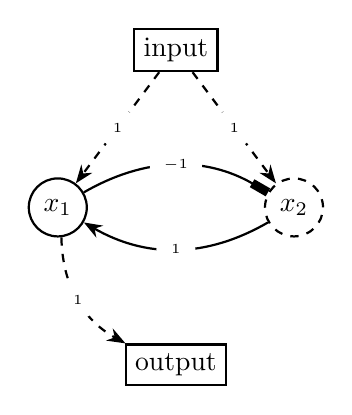
\begin{tikzpicture}
            \begin{scope}[every node/.style={circle,thick,draw}]
                \node (A) at (0,0) {$x_{1}$};
                \node[dashed] (B) at (3,0) {$x_{2}$};
                \node[shape=rectangle] (U) at (1.5,2) {input};
                \node[shape=rectangle] (y) at (1.5,-2) {output};
            \end{scope}

            \begin{scope}[>={Stealth[black]},
                          every node/.style={fill=white,circle},
                          every edge/.style={draw=black, thick}]
                \path [->, >=Rectangle] (A) edge[bend left] node {\tiny $-1$} (B);
                \path [->] (B) edge[bend left] node {\tiny $1$} (A); 
                \path[->] (U) edge[dashed] node {\tiny $1$} (A);
                \path[->] (U) edge[dashed] node {\tiny $1$} (B);
                \path[->] (A) edge[dashed,bend right] node {\tiny $1$} (y);
            \end{scope}
            \begin{scope}[>={Stealth[black]},
                          every edge/.style={draw=black, thick}]
                %\path [->] (A) edge[loop left] node {\tiny $\lambda_{1}$} (A);
                %\path [->] (B) edge[loop left] node {\tiny $\lambda_{2}$} (B);
            \end{scope}

            \end{tikzpicture}
        \end{center}
        \caption{
            Diagram of Example \ref{ex:osc} in the text.  
            \plr{explain what arrows mean if nec}
            \label{fig:oscillator_diagram}}
    \end{figure}

as a special case of the below.

\end{example}


\begin{example}[Example: two-component systems.] \label{ex:2x2}
As a more general example,
suppose that a cell produces two molecular species, $S_1$ and $S_2$ 
whose production are both stimulated by the presence of an external ``input'' substance.
\plr{call them TF?}
Suppose that the two species self-regulate with strengths $\lambda_1$ and $\lambda_2$, respectively,
and the second species also regulates the first species with strength $\gamma$.
\plr{Rephrase in terms of binding to promoter sequences?}
However, only the time course of the concentration of
the first one of these species determines the fitness of the organism.
(As happens for instance in \plr{XXX}.)
Write $x(t) = (x_1(t),x_2(t))$ for the concentrations of the two species at time $t$,
and write $u(t)$ for the concentration at time $t$ of the input substance.
Then, if the rates at which each species are produced
are linear functions of the concentrations
\plr{(look up way this is usually said in the literature.)},
then the dynamics of the system are given by
\begin{align*}
    \ddt x_1(t) &= \lambda_1 x_1(t) + \gamma x_2(t) + u(t) \\
    \ddt x_2(t) &= \lambda_2 x_1(t) + u(t) ,
\end{align*}
where $\ddt x$ denotes the time derivative.
The initial conditions, $x_1(0)$ and $x_2(0)$, 
and the input $u(t)$ then determine the concentrations through time.
If we record the regulatory coefficients in the matrix:
\begin{align*}
    A &= \left[\begin{matrix} 
        \lambda_1 & \gamma \\ 
       0 & \lambda_2  
    \end{matrix}\right],
\end{align*}
and define the column vector $B = [1,1]^T$,
then in matrix notation the dynamics are
\begin{align*}
    \ddt x(t) &= A x(t) + B u(t) .
\end{align*}
If these are all transcription factors,
and we suppose their binding motifs are fixed,
then the $i^\text{th}$ row of $A$ is determined by the $i^\text{th}$ promoter sequence.

\end{example}

Since the system is linear, the state of the system at any time
is the superposition of its responses to all previous inputs.
This implies that 
if $G(t)$ is the transient response of the system to a unit impulse,
$t$ units of time later,
and $x(0) = 0$,
then the time course of the concentration of the thing we care about, $x_1(t)$, 
can be written as
\begin{align} \label{eqn:ex_convolution}
    x_1(t) &= \int_0^t G(t-s) u(s) ds .
\end{align}
However, it turns out that 
\plr{look for simple demontration this is true}
\begin{align*}
    P_{p} = \left[\begin{matrix} 
        1 & 0 \\ 
        p & 1-p 
    \end{matrix}\right],
\end{align*}
then for any $p \neq 1$, 
if we replace the regulatory matrix $A$ with
\begin{align*}
    A(p) = P A P^{-1},
\end{align*}
then the response of $x_1(t)$ to any particular input $u(t)$ is identical to the original system.
(However, $x_2$ may well be different!)

For instance, setting $p=-1$,
the system with
\begin{align*}
    A(-1) = \left[\begin{matrix} 
        \lambda_1 + \gamma/2 & \gamma/2 \\ 
        \lambda_2-\lambda_1-\gamma/2 & \lambda_2 - \gamma/2
    \end{matrix}\right],
\end{align*}
looks very different, but gives the same input-output relationship.
Although these systems are equivalent,
hybrids between them may not be:
\plr{do example}.

\begin{example}[Hyrbid Inviability]
  Let, \begin{align*}
    A(0) =\left[\begin{matrix}
      0 & 1 \\
      -1 & 0
    \end{matrix}\right]
    \text{and }
    A(2) = \left[\begin{matrix}
      2 & -1 \\
      5 & -2
    \end{matrix}\right]
  \end{align*}
  from Example \ref{ex:osc} ($B=\begin{bmatrix} 1 \\ 1 \end{bmatrix}$ and $C=\begin{bmatrix} 1 & 0 \end{bmatrix}$). 
If hybrids are formed by exchanging genes (swapping rows), the hybrid's gene network is,
  \begin{align*}
    \text{hybrid network } := \mathcal{H}(A(0), A(2)) = \left[\begin{matrix}
      2 & -1 \\
      -1 & 0
    \end{matrix}\right] ,
  \end{align*}
  \jss{ Or should it be: \begin{align*}
    \text{hybrid network } := \text{mean}(A(0), A(2)) = \left[\begin{matrix}
      1 & 0 \\
      2 & -1
    \end{matrix}\right] ,
  \end{align*} }
  It's transfer function will be $H(z, \mathcal{H}) = \frac{z-2}{z^2 - 3z +1}$, which produces very different dynamics than its parents, $H(z, A(0)) = H(z, A(2)) = \frac{z+1}{z^2 + 1}$. The time dynamcs of molecular species $1$ in the hybrid is $y^{(\mathcal{H})} =e^{t} \cosh(\sqrt{2} t)$ \jss{ which is approx. $\approx e^{t}$}, with the concentration of species $1$ rapidly heading towards infinity. The dynamics of species $1$ in the parental networks is $y = \sin(t) + \cos(t)$, where it continuously oscillates.

  \jss{The transfer function $H(z, \mathcal{H})$, by averaging networks, is $\frac{1}{z-1}$ and the time dynamics are: $y^{(\mathcal{H})} = e^{t}$.}
\end{example}

\begin{figure}
  \centering
  \begin{subfigure}{0.5\textwidth}
    \centering
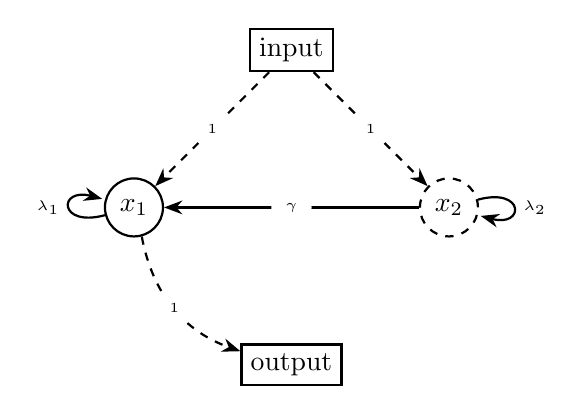
\begin{tikzpicture}
\begin{scope}[every node/.style={circle,thick,draw}]
  \node (A) at (0,0) {$x_{1}$};
    \node[dashed] (B) at (4,0) {$x_{2}$};
    \node[shape=rectangle] (U) at (2,2) {input};
    \node[shape=rectangle] (y) at (2,-2) {output};
\end{scope}

\begin{scope}[>={Stealth[black]},
              every node/.style={fill=white,circle},
              every edge/.style={draw=black, thick}]
    %\path [->] (A) edge[bend left] node {$c$} (B);
    \path [->] (B) edge node {\tiny $\gamma$} (A); 
    \path[->] (U) edge[dashed] node {\tiny $1$} (A);
    \path[->] (U) edge[dashed] node {\tiny $1$} (B);
    \path[->] (A) edge[dashed, bend right] node {\tiny $1$} (y);
\end{scope}
\begin{scope}[>={Stealth[black]},
              every edge/.style={draw=black, thick}]
    \path [->] (A) edge[loop left] node {\tiny $\lambda_{1}$} (A);
    \path [->] (B) edge[loop right] node {\tiny $\lambda_{2}$} (B);
\end{scope}

\end{tikzpicture}
    \caption{Gene Regulatory Network $A(0)$.}
  \end{subfigure}%
  \begin{subfigure}{0.5\textwidth}
    \centering
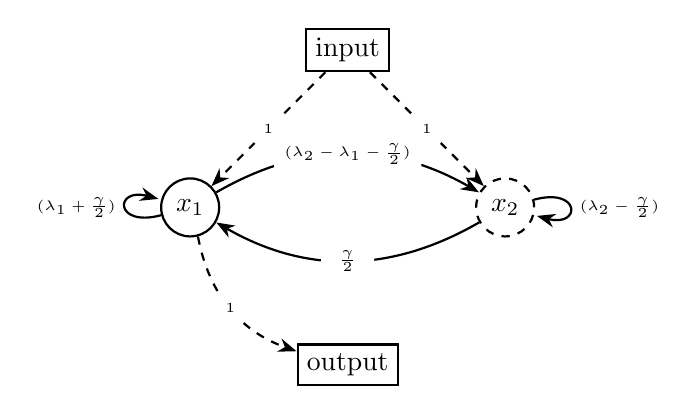
\begin{tikzpicture}
\begin{scope}[every node/.style={circle,thick,draw}]
  \node (A) at (0,0) {$x_{1}$};
    \node[dashed] (B) at (4,0) {$x_{2}$};
    \node[shape=rectangle] (U) at (2,2) {input};
    \node[shape=rectangle] (y) at (2,-2) {output};
\end{scope}

\begin{scope}[>={Stealth[black]},
              every node/.style={fill=white,circle},
              every edge/.style={draw=black, thick}]
    \path [->, sloped] (A) edge[bend left] node {\tiny $(\lambda_{2} - \lambda_{1} - \frac{\gamma}{2})$} (B);
    \path [->, sloped] (B) edge[bend left] node {\tiny $\frac{\gamma}{2}$} (A); 
    \path[->] (U) edge[dashed] node {\tiny $1$} (A);
    \path[->] (U) edge[dashed] node {\tiny $1$} (B);
    \path[->] (A) edge[dashed, bend right] node {\tiny $1$} (y);
\end{scope}
\begin{scope}[>={Stealth[black]},
              every edge/.style={draw=black, thick}]
    \path [->] (A) edge[loop left] node {\tiny $(\lambda_{1} + \frac{\gamma}{2})$} (A);
    \path [->] (B) edge[loop right] node {\tiny $(\lambda_{2}-\frac{\gamma}{2})$} (B);
\end{scope}

\end{tikzpicture}
    \caption{Gene Regulatory Network $A(-1)$.}
  \end{subfigure}
  \caption{Neutral rewiring of gene network $A(p)$ from Example \ref{ex:2x2}. Not only are the regulatory coefficients different between $A(0)$ and $A(-1)$, there is also a new regulatory connection.}
\end{figure}


\section{Regulatory networks as linear, time-invariant systems}

\plr{Make sure to have strongly worded disclaimer somewhere
that we know real networks aren't linear
but they are locally.
Plus, it works in engineering.}

% - General description of the LTI process in biological context
%     * y = "phenotype"
%     * x = "internal state" or "kryptotype"?
%     * A = "regulatory matrix" or "genetic network"?
% - Why transfer function determines input-output relationship
% - Kalman decomposition in unique form

We will now lay out the model in more general terms.
Suppose that the \emph{internal state} of the system
is parameterized by the concentrations of a collection of $n$ molecular species,
$S_1, \ldots, S_n$,
and the vector of concentrations at time $t$ we denote $x(t)=(x_1(t),\ldots,x_n(t))$.
There are also $m$ ``input'' species, whose concentrations are determined
exogenously to the system,
and are denoted $u(t) = (u_1(t),\ldots,u_m(t))$,
and $\ell$ ``output'' species, whose concentrations are denoted
$y(t) = (y_1(t),\ldots,y_\ell(t))$.
The output is merely a linear function of the internal state:
\begin{align*}
    y_i(t) = \sum_j C_{ij} x_i(t).
\end{align*}
Since $y$ is what natural selection acts on, we refer to it as the \emph{phenotype},
and sometimes in contrast refer to $x$ as the \emph{kryptotype},
as it is ``hidden'' from direct selection.
\plr{Maybe.}
The rate at which the $i^\text{th}$ species is produced
is a weighted sum of the concentrations of the other species
as well as the input:
\begin{align*}
    \ddt x_i(t) = \sum_j A_{ij} x_j(t) + \sum_k B_{ik} u_k(t) .
\end{align*}
In matrix notation, this is written more concisely as
\begin{align} \label{eqn:lti_system}
    \ddt x(t) &= A x(t) + B u(t) \\
    y(t) &= C x(t) .
\end{align}

\plr{Everything we say I think is assuming $x(0)=0)$.  
Figure this out. ``Zero-state equivalence.''}

Given an initial condition and an input, 
it is possible to write the solution $x(t)$
as a convolution with an input-response kernel as in the example above
(equation \eqref{eqn:ex_convolution}).
An alternative way of describing the input-output relationship,
more common in engineering,
is instead to find the \emph{transfer function}
\begin{align} \label{eqn:transfer_fn}
    H(z) = C(z I - A)^{-1} B,
\end{align}
which is more mathematically readable \plr{if you know what it means}.
This can be thought of as the system's response to input at ``frequency'' $z$.
The fact that the transfer function uniquely determines the system's
input-output relationship (i.e., the mapping $u \mapsto y$)
follows from the fact that if $\tilde y(z) = \int_0^\infty e^{-zt} y(t) dt$
is the Laplace transform of $y$,
and $\tilde u(z)$ is the Laplace transform of $u$,
then
\begin{align*}
    \tilde y(z) = H(z) \tilde u(z) .
\end{align*}
(This happens because the Laplace transform takes convolutions to products,
and $H$ is the Laplace transform of the kernel $G$.)
Concretely,

\plr{Should we remind what dimensions everything is?}

The state space representation is considered an internal description of the
system, whereas the transfer function is an external description. 
``Realizations'' are something.

\begin{definition}[Phenomenological equivalence of systems]
    Let $(x(t),y(t))$ and $(\bar x(t),\bar y(t))$ be the solutions to \eqref{eqn:lti_system}
    with coefficient matrices $(A,B,C)$ and $(\bar A,\bar B,\bar C)$ respectively,
    and both $x(0)$ and $\bar x(0)$ are zero. 
    The systems defined by $(A,B,C)$ and $(\bar A,\bar B,\bar C)$ are
    \textbf{phenomenologically equivalent} 
    if
    \begin{align*}
        y(t) = \bar y(t) \qquad \text{for all} \; t \ge 0.
    \end{align*}
    Equivalently, this occurs if and only if
    \begin{align*}
        H(z) = \bar H(z)  \qquad \text{for all} \; z \ge 0,
    \end{align*}
    where $H$ and $\bar H$ are the transfer functions of the two systems.
\end{definition}

One way to find other systems equvalent to a given one
is by change of coordinates (``algebraic equivalance''):
if $T$ is an invertible matrix, then the systems $(A,B,C)$ and $(TAT^{-1},TB,CT^{-1})$
have the same dyanamics because their transfer functions are equal:
\begin{align*}
    CT^{-1}( zI - TAT^{-1})^{-1}TB
    =
    CT^{-1}T( zI - A)^{-1}T^{-1}TB
    =
    C( zI - A)^{-1}B .
\end{align*}
However, the converse is not necessarily true: 
systems can have identical transfer functions without being changes of coordinates of each other.
In fact, systems with identical transfer functions can involve interactions between different
numbers of molecular species.

The set of all systems phenomenologically equivalent to a given system $(A,B,C)$ 
is elegantly described using the Kalman decomposition,
which also clarifies the system dynamics? tells us a lot about how it works? \plr{or something}
To motivate this, first note that the the input $u(t)$ only directly pushes the system
in directions lying in the span of the columns of $B$.
As a result, different combinations of input can 
move the system in any direction that lies in the \emph{reachable subspace},
which we denote by $\reachable$,
and is defined to be the closure of $\spn(B)$ under applying $A$
(or equivalently, the span of $B, AB, A^2B, \ldots A^{n-1}B$).
Analogously to this, we define
the \emph{observable subspace}, $\mathcal{O}$,
to be the closure of $\spn(C^T)$ under applying $A$.
(Or: $\unobservable$ is the largest $A$-invariant subspace
contained in the null space of $C$;
and $\reachable$ is the largest $A$-invariant subspace contained in the image of $B$.)

If we define
\begin{enumerate}
    \item The columns of $P_\rno$ are an orthonormal basis for $\reachable \cap \unobservable$.
    \item The columns of $P_\ro$ are an orthonormal basis of
        the complement of $\reachable \cap \unobservable$ in $\reachable$.
    \item The columns of $P_\nro$ are an orthonormal basis of
        the complement of $\reachable \cap \unobservable$ in $\unobservable$.
    \item The columns of $P_\nrno$ are an orthonormal basis of
        the the remainder of $\R^n$.
\end{enumerate}
If we then define
\begin{align*}
    P &= 
    \left[ \begin{array}{c|c|c|c}
        P_\rno & P_\ro & P_\nro & P_\nrno
    \end{array} \right] ,
\end{align*}
then
\begin{align*}
    P^T P
    &=
    \left[ \begin{array}{c|c|c|c}
        I & 0 & 0 & 0 \\
        \hline
        0 & I & U & 0 \\
        \hline
        0 & V & I & 0 \\
        \hline
        0 & 0 & 0 & I 
    \end{array} \right] .
\end{align*}
\plr{Check this.  Can we get $U=V=0$?}

The following theorem can be found in SOME REFERENCE.

\begin{theorem}[Kalman decomposition] \label{thm:kalman}
        For any system $(A,B,C)$ with corresponding Kalman basis matrix $P$,
        the transformed system $(PAP^{-1},PB,CP^{-1})$  has the following form:
        \begin{align*}
            \widehat A = PAP^{-1}
            &=
            \left[ \begin{array}{cccc}
                A_{\rno} & A_{\rno,\ro} & A_{\rno,\nrno} & A_{\rno,\nro} \\
                0 & A_{\ro} & 0 & A_{\ro,\nro} \\
                0 & 0 & A_{\nrno} & A_{\nrno,\nro} \\
                0 & 0 & 0 & A_{\nro}
            \end{array} \right] ,
        \end{align*}
        and
        \begin{align*}
            \widehat B = PB
            &=
            \left[ \begin{array}{cccc}
                B_{\rno} \\
                B_{\ro} \\
                0 \\
                0 
            \end{array} \right] ,
        \end{align*}
        and
        \begin{align*}
            \widehat C = CP^{-1}
            &=
            \left[ \begin{array}{cccc}
                0 & C_{\ro} & C_{\nrno} & 0 
            \end{array} \right] .
        \end{align*}
        The transfer function of both systems is given by
        \begin{align*}
            H(z) = C_{\ro} ( zI - A_{\ro} )^{-1} B_{\ro} .
        \end{align*}
\end{theorem}

In the latter case, we say that the system is \emph{minimal} 
-- there is no equivalent system with a smaller number of species.
Note that this says that any two equivalent minimal systems
are changes of basis of each other.

Since any system can be put into this form,
and once in this form, its transfer function is determined only by 
$C_{\ro}$, $A_{\ro}$, and $B_\ro$,
therefore, the set of all equivalent systems are parameterized by
the dimension $n$,
the choice of basis ($P$),
the remaining submatrices in $\widehat A$, $\widehat B$, and $\widehat C$
(which are unconstrained),
and a invertible transformation of $\spn(P_{\ro})$, which we call $T_\ro$.

\begin{theorem}[Parameterization of equivalent systems]
    Let $(A,B,C)$ be a minimal system.
    \begin{itemize}
        \item[(a)]
            Every equivalent system is of the form given in Theorem \ref{thm:kalman},
            i.e., can be specified by choosing a dimension, $n$;
            submatrices in $\widehat A$, $\widehat B$, and $\widehat C$ 
            except for $A_\ro=A$, $B_\ro=B$, and $C_\ro=C$;
            and choosing an invertible matrix $P$.

        \item[(b)]
            \plr{conjecture:}
            The parameterization is unique
            if $P$ is futhermore chosen so that 
            each $P_x$ other than $P_\ro$ is a projection matrix,
            and that 
            \begin{align*}
                0
                =
                P_x^T P_y
            \end{align*}
            for all $(x,y)$ except $(\ro,\nrno)$.

    \end{itemize} 
\end{theorem}

\plr{Another way of saying it: pick the $\reachable$ and $\unobservable$ subspaces,
that must intersect in something of the minimal dimension;
then let $P$ be the appropriate basis?}

In some situations we may be interested in only ``network rewiring'',
where $A$ changes while $B$ and $C$ do not.
For instance, 
if all non-regulatory functions of each molecule are strongly constrained,
then $C$ cannot change.
Likewise, if responses of each molecule to the external inputs are not changed by evolution,
then $B$ does not change.

\begin{lemma}
    Let $(A,B,C)$ be a system.
    Every matrix $\widehat A$ such that $(\widehat A,B,C)$ is equivalent to $(A,B,C)$
    can be specified in the form given in Theorem \ref{thm:kalman},
    with \plr{them having the same $\ro$ bit}
    and satisfying
    \begin{align*}
        \widehat B &= P B \\
        \widehat C P &= C
    \end{align*}
\end{lemma}

It is remarkable to note that even with the relationships 
between environment, cryptotype, and phenotype constant,
and in the minimal dimension,
there are still almost always degrees of freedom.
These correspond to distinct genetic networks
that perform indistinguishable functions.
For example, the equivalent systems of Example \ref{ex:2x2} above
are minimal, and share common $B$ and $C$ matrices.

\plr{Maybe say that stability to noise can be determined by $A_\nro$ (and others?),
while complexity of the internal, unobserved dynamics
are somehow given by the difference between the dimension of $y$ and the dimension of $A_\ro$.}

\plr{General argument why Brownian motion on set of equivalent things is maybe ok.}

\begin{example}
    The system in Example \ref{ex:2x2} is minimal, so $A=A_\ro$,
    and the only free parameter is $P$.
    Suppose also that the effects of the input and output are strongly constrained,
    so that as in that example,
    $B$ and $C$ cannot change,
    and neutral evolution moves through the set of of $P$ such that $PB=B$ and $CP=C$.
    \plr{Clarify we mean with no gene duplication and only neutral drift.}
    How will this system change over evolutionary time in the manner described \plr{above}?
    An unbiased Brownian motion on this set 
    can be written in terms of a one-dimensional Brownian motion $\beta_\tau$ 
    with $\beta_0=0$ as
    \begin{align*}
        P(\tau) = \left[
            \begin{array}{cc}
                1 & 0 \\
                e^{\beta_\tau}-1 & e^{\beta_\tau}
            \end{array}
            \right] .
    \end{align*}
    Therefore, the state of the system after (evolutionary) time $\tau$
    is $(P(\tau)AP(\tau)^{-1},B,C)$.
\end{example}


\section{What biological question are we asking?}

How do gene regulatory networks (GRNs) change through evolutionary time?
Specifically, under constant selection and environmental pressures, how does a
maximally fit population's GRN change and what molecular and population
parameters are significant to the process? How frequent does gene network
rewiring occur in the absense of genetic drift or adaptation? Is rewiring
typically compensatory and ususally follow the fixation of a deleterious
allele, or can networks neutrally reorganize? How does the size, average
degree, function, peiotropy, etc of a network influence its likelihood to
drift? If networks can drift, how much topological heterogeneity can a
well-mixed population tolerate, if any? Does topoligical heterogeneity and/or
the size of the neutral genotype-set, if consequences of network organization,
constrain or entail exaptation and evolvability? Are some network organizations
(maybe higher dimensional realizations?) able to more rapidly evolve to
construct novel phenotypes and meet the demands of changes in selection
pressures?

\section{How can we mathematically model this question?}

In some respect an organism can be thought of as a black box that responds to
some set of inputs (it's environment and other initial conditions) and outputs
a phenotype. The phenotype is then evaluated by natural selection. The black
box metaphor holds, because much of the details of what happens to construct a
phenotype are unimportant as far as selection is concered, so long as the
phenotype reliably performs its function. If multiple internal mechanisms can
map the same set of inputs to the same set of outputs, and these mechanisms are
mutationally nearby (in genotype space), then evolution may drift from
mechanism to mechanism. 

In this simple model we can say that $B\vec{u}$ is a list of initial GRN
protein concentrations determined by the more general initial environmental
conditions $\vec{u}$. $A$ represents all the genetic interactions of a
particular GRN, and $C\vec{x}$ is an organism's phenotype. Fitness could be
calculated by comparing a subset of the phenotype to an optimum. Maybe,
$f(\cdot) = e^{- \int_{a}^{b} \Vert G(s) - G^{*}(s) \Vert ds}$ Alternatively,
fitness scores could simply assess whether or not a phenotype is within some
range or breaks some threshold by some time point. Or possbily the simplest:
any phenotype not exactly equal to $G(s)$ is lethal, and $G(s)$ is perfectly
fit. 

Next, we will have to define mutation and recombination. Mutation needs to add
and remove genetic interactions and recombination needs to shuffle genes during
sexual reproduction. We could adapt methods from Lynch 2007 and Lynch and
Hagner 2015 to model the probability of a TFBS appearing or disappearing due to
mutational pressure. Every time a new binding site is gained or lost, the
values within the A matrix are either modified or rows and columns are added
removed following a specific set of rules. I am not sure if it would be easier
to maintain a matrix size (say $m \times m$) where $m$ is arbitrarily large,
with  most entries being zero, or if a matrix should only have as many
dimensions as the number of active TFs. Recombination should then shuffle rows
of the $A$ matrix randomly, as each row represents the regulatory region of a
given gene (assuming only cis-regulation, and that the regulatory element is
small enough to not break up during recombination).  

To study some of the above posed questions, we can simulate (or analytically
determine) the rates of GRN change, and how frequently these changes lead to
significant rewiring or speciation. We would want to know the dynamics of a
brownian motion over the set of all realizations.  Another interesting question
would be to determine the size of the neutral genotype space as well as the
number of connections from the neutral genotype space to the non-neutral
genotype space. Maybe higher dimensional realizations of a GRN will have
significantly more connections to non-neutral genotypes and therefore be more
``evolvable'' or exapted to novel environments? 

Let $M \in \mathbb{R}^{n \times n}$ be a least dimensional realization of $A$,
and let $M'$ bean $(n+m \times n+m)$ matrix where $M'_{(i,j)} = M_{(i,j)} \
\text{for } i,j \leq n, \ \text{and } 0 \ \text{otherwise}$. Let $P$ be any
$(n+m \times n+m)$ matrix with rank $n$. Then for any matrix $B$ such that $BP
= PM'$, $B$ is a realization of $A$.     

\section{List of papers with some notes.}

R. E. Kalman, “Mathematical description of linear dynamical systems,” Journal of the Society for Industrial and Applied Mathematics, Series A: Control, vol. 1, no. 2, pp. 152–192, 1963.
This is a good overview written by Kalman. Probably the most important paper on this list.

Minimal state-space realization in linear system theory: an overview. B. De Schutter. 2000.
Another, more recent, overview that I found helpful to understand controllability and observability. 

The Inverse Problem of Stationary Covariance Generation. BDO Anderson. 1969.

Equivalence of Linear Time- Invariant Dynamical Systems. BDO Anderson, BW Necomb, RE Kalman. 1966. 

B. Ho and R. E. Kalman, “Effective construction of linear state-variable models from input/output functions,” Proceedings of the 3rd Annual Allerton Conference on Circuit and System Theory, vol. 1, no. 2, p. 449459, 1965.

Dynamic Structure Functions for the Reverse Engineering of LTI Networks. J Goncalves. 2007.
I have not read this paper yet, but apparently it outlines a method for recovering the state space equation from specific sets of measurements.

New Developments in Systems Theory Relevant to Biology. RE Kalman. 1968.
Not technical but kind of interesting. 

Old and New Directions of Research in Systems Theory. RE Kalman. 2010?

Minimality and Observability of Group Systems. HA Loeliger, GD Forney Jr., T Mittelholzer, MD Trott. 1994. 
Another paper I just found. It looks like it might be useful.

Partial Realization of Descriptor Systems. P Benner and VI Sokolov. 2006. 
I think this is about recovering a finite realization from infinite systems. Maybe it would be interesting to think about the similarity between transfer functions though? If selection only cares about a specific interval of the transfer function, say $G(10)$, then maybe two partial transfer functions will be effecrively equivlaent? 

There are also the previous papers I sent on identifiability and distinguishability. In the original Bellman and Astrom paper where they introduce ``structural identifiability'' they show that a linear dynamical system is identifiabile if and only if it is also controllable and observable. 


\section{Notes on what to do when allowing deleterious mutations}

Epistasis, coming from mutations deleterious in some networks but not in others
(come from incompatibilities).

Describe heterosis.

Distribution of dominance coefficients.

\bibliographystyle{plainnat}
\bibliography{krefs}


\end{document}
